\section{空间解析几何}

\subsection{作业}

\begin{problem}
	习题一
	\begin{solution}
		原曲线方程即为
		$$
		x = \frac{y^2}{2} + \frac{9}{2},\ z = 3
		$$
		点 $(x, y, z)$ 在 $xOy$ 上的投影是 $(x, y, 0)$。因此投影曲线方程为
		$$
		x = \frac{y^2}{2} + \frac{9}{2},\ z = 0
		$$
		原曲线和投影后的曲线都是一个抛物线。
	\end{solution}
\end{problem}

\begin{problem}
	习题二
	\begin{solution}
		\begin{enumerate}
			\item[\textbf{1)}] 这个曲面是一个椭圆抛物面。
			\item[\textbf{2)}] 这个曲面是一个椭圆双曲面。
			\begin{figure}[H]
				\centering
				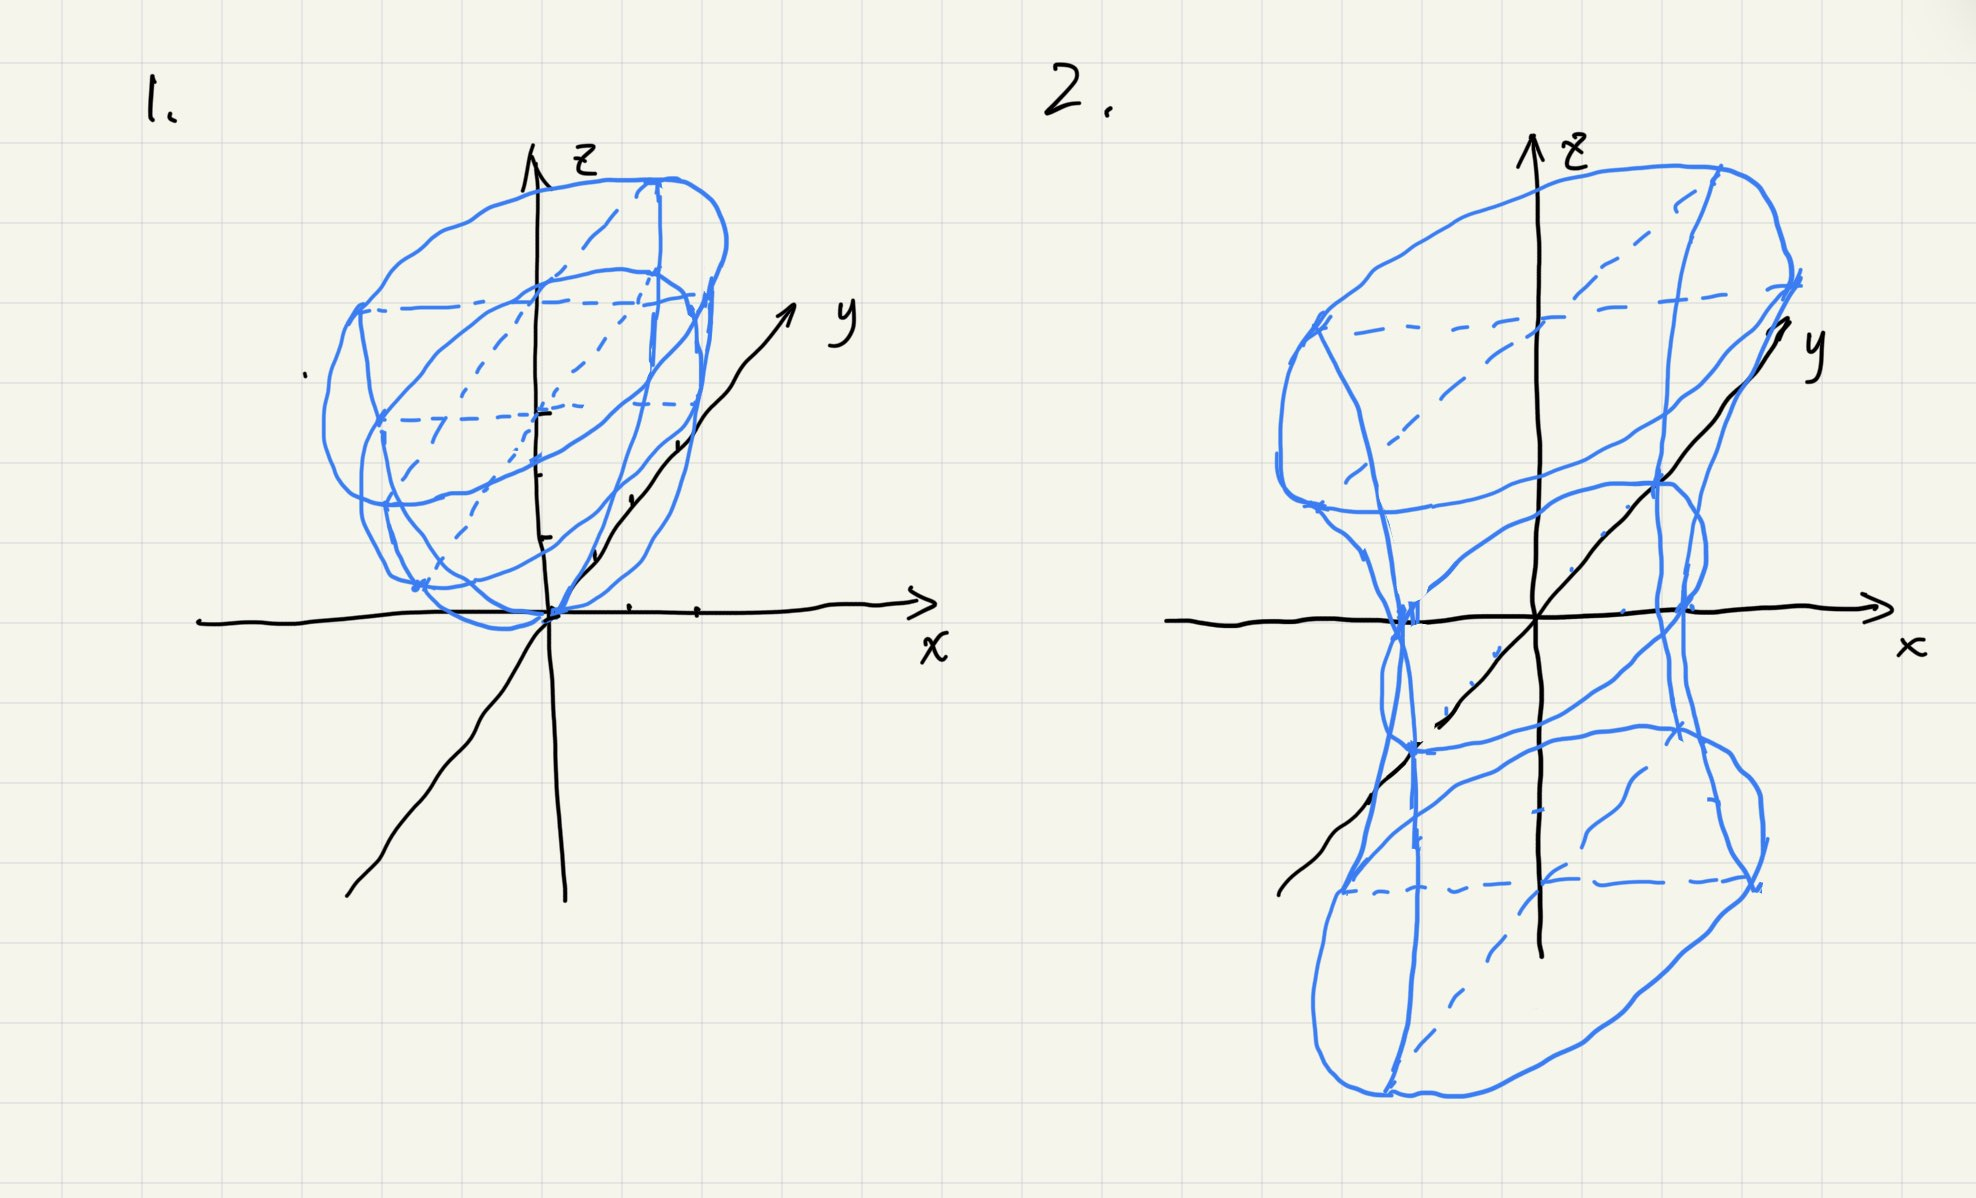
\includegraphics[scale=0.15]{线性代数应用案例选讲/graphics/answer1.png}
			\end{figure}
		\end{enumerate}
	\end{solution}
\end{problem}

\begin{problem}
	习题三
	\begin{solution}
		\ 
		\begin{figure}[H]
			\centering
			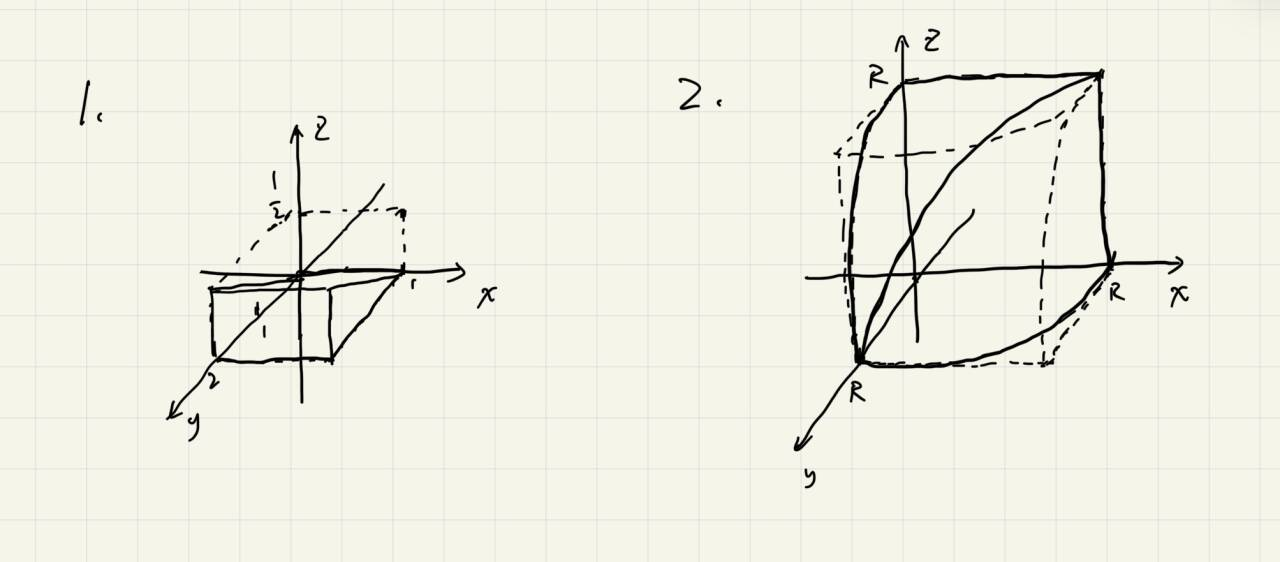
\includegraphics[scale=0.22]{线性代数应用案例选讲/graphics/answer2.png}
		\end{figure}
	\end{solution}
\end{problem}

\begin{problem}
	习题四
	\begin{solution}
		\begin{itemize}
			\item 用平面 $z = h$ 截得到
			$$
			-\frac{x^2}{2p} + \frac{y^2}{2q} = h
			$$
			$h \neq 0$ 时这是一条双曲线，$h = 0$ 时这是两条相交直线。

			\item 用平面 $x = k$ 截得到
			$$
			z = \frac{y^2}{2q} - \frac{k^2}{2p}
			$$
			这是一条开口向上的抛物线，且顶点随 $k$ 增大而下降。

			\item 用平面 $y = m$ 截得到
			$$
			z = -\frac{x^2}{2p} + \frac{m^2}{2q}
			$$
			这是一个开口向下的抛物线，且顶点随 $m$ 增大而上升。
		\end{itemize}

		可知这个曲面被称为双曲抛物面，即马鞍面。

		\begin{figure}[H]
			\centering
			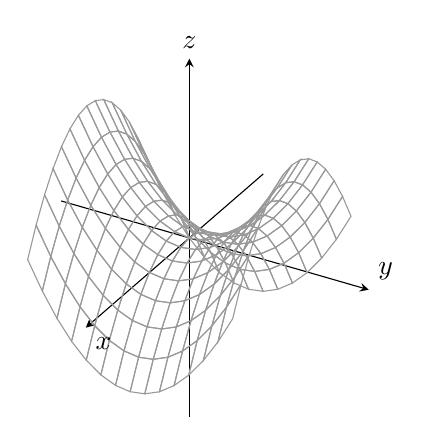
\begin{tikzpicture}
				\begin{axis}[
					view={120}{30},
					axis lines=center,
					xmin=-2.5, xmax=3.5,
					ymin=-2.5, ymax=3.5,
					zmin=-3.5, zmax=3.5,
					xlabel={}, ylabel={}, zlabel={},
					ticks=none,
					axis equal image,
					clip=false,
					scale=2,
				]
					\addplot3[
						mesh,
						shading=none,
						color=black!40,
						samples=15,
						domain=-2:2,
						y domain=-2:2,
					] { (y^2)/2 - (x^2)/2 };
					\node[anchor=north west] at (axis cs: 3.5, 0, 0) {$x$};
					\node[anchor=south west] at (axis cs: 0, 3.5, 0) {$y$};
					\node[anchor=south]      at (axis cs: 0, 0, 3.5) {$z$};
				\end{axis}
			\end{tikzpicture}
			\caption{双曲抛物面}
		\end{figure}
	\end{solution}
\end{problem}